\subsection{Specifying and Inferring Probability Distributions}
\label{sec:probspecs}

\begin{figure}
\centering
      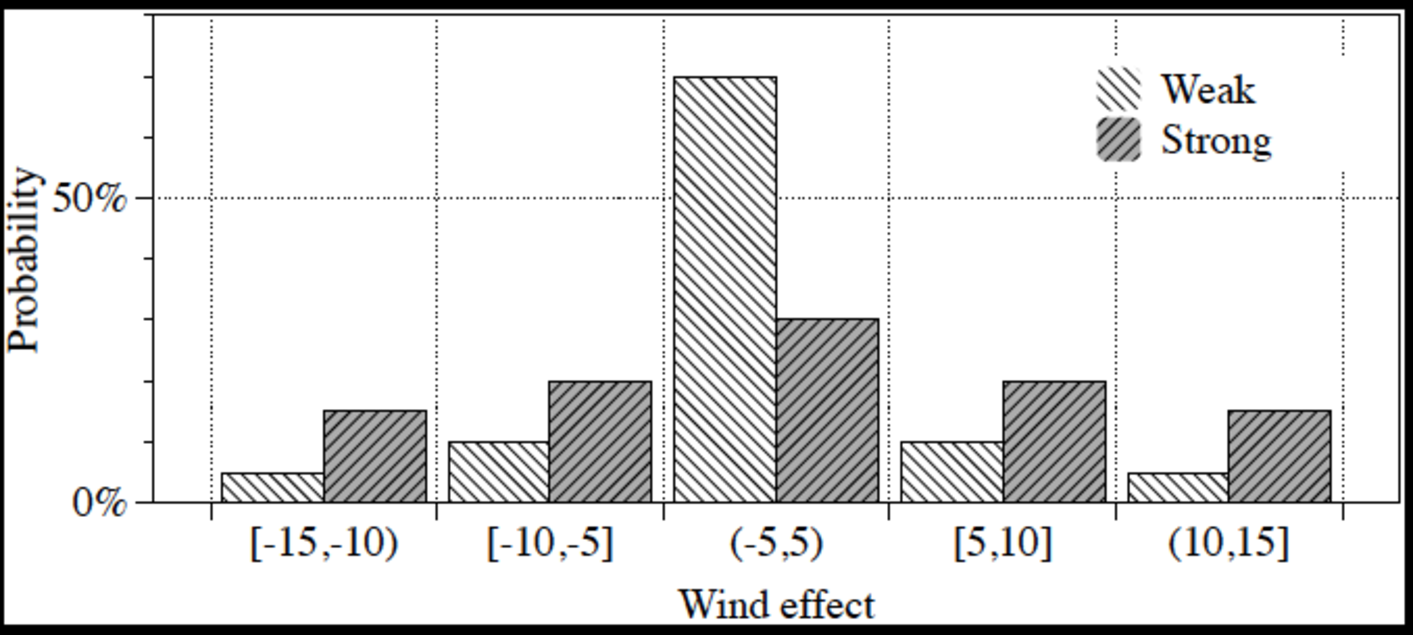
\includegraphics[width=10cm]{up}
\caption{Example Usage Profile}
\label{fig:up}
\end{figure}


The probabilistic symbolic execution defined in the previous section
makes use of a probabilistic {\em usage profile}, which is an estimate
of the probability distribution of a program's input space.  Usage
profiles can be {\em specified} based on physical phenomena, known
sensor parameters, or other domain-specific knowledge about the program
and its deployment context.  

In our initial work, we handled arbitrary probabilistic usage profiles through discretization. For example, Figure~\ref{fig:up} illustrates two "discretized" usage profiles representing strong and weak wind conditions. Such usage profiles can be used for e.g. analyzing the wing controller of an aircraft under different wind conditions. The ranges of values for the wind effect are reported on the x-axis, and the corresponding vertical bars represent the probability of a value in the range to be inserted as input. In this example, we assume symmetric distributions for the two profiles. Weak wind is more concentrated around zero, while strong wind is more likely to produce extreme values.


Usage profiles can also be {\em built}
automatically based on observed data from past usages of the program.
Finally, best(worst)-case usage profiles can be {\em inferred} from
the structure of a program itself.  

\subsubsection{Building usage profiles from observed data}
It is possible to obtain usage profiles systematically from
telemetry data, log files, and simulation
data available from previous or similar usages (missions) of 
the software under analysis.
For example, one can measure
the frequency of values occurring within certain ranges
during a mission to obtain realistic usage profiles. 
Furthermore, as in the case of probabilistic
programming~\cite{Gordon2014}, the code can also be
used to formalize the dynamics of a system, from biological processes
to financial markets. In these cases, probabilistic profiles can 
either be inferred through the analysis of experimental or historical
data or be deduced from physical laws.


In the simplest case, operational profiles can be inferred from raw
data by measuring the frequency or proportion of the observed data
within pre-specified ranges.  This gives an estimation of the
distribution of the data for the duration the system was observed.
Such profiles can then be used to assess the probabilistic properties
of a new version of the system, or of a similar system.


In addition to the usage profiles that specify the distributions of
the input data~\cite{Filieri2013}, one can use stateful usage profiles
given as Discrete-Time Markov Chains (DTMC), for example.  Such
profiles are useful for the class of systems that typically operate on
sequences of inputs---so-called reactive programs.

To apply probabilistic analysis to such systems, one must extend both
the usage profiles and the probability computation to consider input
values and probability distributions that are correlated with previous
inputs in the environment.  Conceptually, the DTMC generates a
\textit{driver} that interacts with the analyzed software according to
the distribution.

Informally, DTMC are automata labeled with outgoing probabilities on
their transitions.  DTMC are already a common formalism for expressing
probabilistic usage models, and we can employ inference procedures to
build them automatically.  Such inference was presented in
e.g. \cite{ghezzi2014mining,beschastnikh2011leveraging}). The procedures consume logged data
which typically consists of a time series, where each log entry encodes the value
of the states observed at each time step. The states of the inferred
model then represent ``abstractions'' of the state reported in the log
file, and transitions in the model correspond to the time steps in the
log file. The abstraction is defined by the user and it depends on the
properties of interest. The log data is discretely sampled, in some
cases many times per second, therefore it is necessary to select a
resolution to allow for more realistic state transitions and to
prevent state space explosion. The probability distribution for a
particular state $s$ is estimated by computing the ratio between the
number of traversals for each outgoing transition and the total number
of traversals of the transitions exiting state $s$; this corresponds
to the {\em maximum likelihood estimator} for the probability
distribution at that state.

An alternative is to explore Bayesian inference---a method of
statistical inference in which Bayes' rule is used to update the
probability estimate for a hypothesis as additional evidence is
acquired. Bayesian updating is an important technique throughout
statistics, and especially in mathematical statistics. For some cases,
exhibiting a Bayesian derivation for a statistical method
automatically ensures that the method works as well as any competing
method. Bayesian updating is especially important in the dynamic
analysis of a sequence of data. This is a topic for future work.


\subsubsection{Inferring best/worst-case usage profiles}
There may be cases where developers have little, or no, basis for
formulating or validating a usage profile.  An interesting topic for
future research is the automatic inference of {\em symbolic usage
  profiles} to provide a mechanism for explicitly encoding the lack of
knowledge about user inputs---through the use of symbolic variables
to denote the mass in a region of the input space, $m_i$.

For this approach, one can fix the shape of the
distribution (e.g., the bins of a histogram estimator, the states of a
Markov chain) and then use probabilistic analysis to encode
constraints among mass values in the regions of the distribution.  
For example, from observed data, developers might be
very confident that values in the range $[10,30]$ are at least two
times more likely than values in the range $[30,60]$.  This can be
encoded as an \textit{intra-distribution constraint}, $m_1 + m_2 >
2(m_3 + m_4 + m_5)$, where $m_i$ are the variables for five bin masses
between 10 and 60.

Probabilistic analysis could compute for each path, $p_i$,
the quantity $\Sigma_{j} \#(C_i \wedge b_j)*m_j$, where $b_j$ are discrete
regions of the distribution estimator.  Wherever the mass
of that region is known, $m_j$ is a constant, otherwise it is
a free variable modeling an unknown mass.

Upon completion of the analysis, the following sum
$\Sigma_{j} (\Sigma_i \#(C_i \wedge b_j)) *m_j$
forms the basis for an optimization problem.
Minimizing this sum, subject to the constraints  
$\Sigma_j = 1$ and any intra-distribution constraint, gives
the values for $m_j$ that lead to the lowest confidence in
system behavior---a worst-case usage profile.  The best-case
is similar except that the sum is maximized.

When intra-distribution constraints are linear, this results
in a linear programming problem.  There are numerous efficient solvers
for these problems, e.g., CPLEX \cite{cplex2009v12}, that are known to
support upward of a billion variables---subject to sufficient memory.
For many systems, we expect that the existence of partial distribution
information
will significantly reduce the number of symbolic variables required,
and thus, systems with 10s of input variables can be handled
directly with off-the-shelf solvers. 

For the general (non-linear) case, one can explore {\em learning
  techniques}, such as reinforcement learning or Monte-Carlo
tree-search~\cite{sutton1998reinforcement} to iteratively compute
best/worst usage profiles with respect to desired properties. We have
already explored reinforcement learning in~\cite{luckow2014exact} to
infer best/worst schedules in the context of probabilistic analysis of
concurrent programs. A similar approach can be applied to profile
inference as well. 

\ignore{
Note that our discussions about generalizing the work from ASE 2014 
also aims to fix the structure of an MDP describing the time-series
input structure of the environment.  The probability distributions
governing nondeterministic transitions in that MDP are inferred,
using a different technique, to compute angelic (demonic) usage
profiles.
}

